\documentclass{article}
\usepackage[a4paper,left=10mm,right=10mm,top=15mm,bottom=15mm]{geometry}
\usepackage{amssymb,amsthm,latexsym,amsfonts, amsmath}
\usepackage[noeepic]{qtree}
\usepackage{tikz}
\usetikzlibrary{backgrounds}
\usetikzlibrary{trees,positioning,arrows}
\usepackage{extarrows}
\usepackage{german}
\title{Übungen zur Algorithmischen Bioinformatik I\\
Blatt 4}
\author{Xiheng He}
\date{Mai 2021}
\linespread{1.8}
\begin{document}
\maketitle
\begin{flushleft}
\textbf{2. Aufgabe (10 Punkte):}\\
wenden Sie das Master-Theorem an um die Laufzeit für folgende Rekursionsgleichungen zu bestimmmen (mit T(1) = 1) oder begründen Sie, warum das Master-Theorem nicht anwendbar ist.
\newline
Master-Therorm: $T(n) = a \cdot T(n/b) + f(n)$ für $n > 1$ und $T(1) = d$. dann gilt:
    $$ T(n)=\left\{
    \begin{aligned}
    &\Theta(n^{\log_b (a)}) & falls \; f(n) = O(n^{\log_b (a)-e}), e > 0 \\
    &\Theta(n^{\log_b (a)}\log(n)) & falls \; f(n) = \Theta(n^{\log_b(a)})\\
    &\Theta(f(n)) & falls \; f(n) = \Omega(n^{\log_b(a) + e}), e > 0 \; und \; a \cdot f(n/b) \le c \cdot f(n), c < 1\\ 
    \end{aligned}
    \right.
    $$
\newline
(a) $T(n) = 3 \cdot T(n/4) + n$
\newline
aus (a) ist $f(n) = n, a = 3, b = 4$
\newline
$\log_b(a) = \log_4 3 \approx 0.792$
\newline
da $n^{log_4 3} < f(n)=n \ \forall  \ n > 1$ handelt es sich um den dritten Falls des Mastertheorems.
\newline
Deshalb muss 2.Eigenschaft validiert werden: $a\cdot f(n/b) \leq c\cdot f(n)$
\newline
$3\cdot (n/4)= \frac{3 \cdot n}{4}= \frac{3}{4}\cdot n$
\newline
$\Longrightarrow$ Der 3. Fall gilt mit $c=\frac{3}{4}<1$ und $T(n)=\Theta(f(n))=\Theta(n)$
\newline\\
(b) $T(n) = 3 \cdot T(n/4) + \sqrt{n}$
\newline
aus (a) ist $f(n) = \sqrt{n}, a = 3, b = 4$
\newline
$\log_b(a) = \log_4 3 \approx 0.792$
\newline 
es gilt der erste Fall, da gilt :
\newline
$f(n)=\sqrt{n} \in \theta (n^{log_4(3)-\varepsilon}) $
\newline
da für ein $\varepsilon > 0$ z.B.$\varepsilon =0.2$ immer noch gilt $n^{log_4(3)-\varepsilon}=n^{0.392} \ge \sqrt{n} $
\newline
$\Longrightarrow T(n)= \theta (n^{log_43})$
\newpage
zu a)
\newline
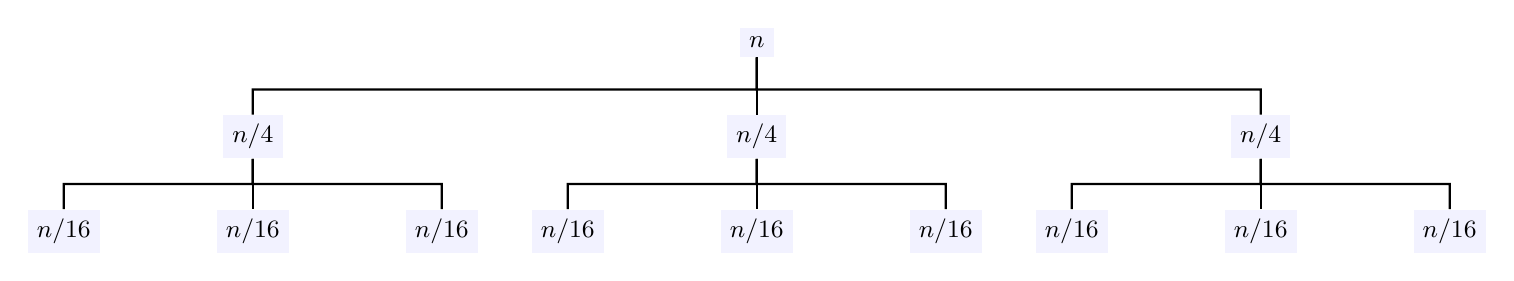
\begin{tikzpicture}[scale=0.8,font=\small, edge from parent fork down,
every node/.style={fill=blue!5},
edge from parent/.style={black,thick,draw},
level 1/.style={sibling distance=8cm},
level 2/.style={sibling distance=3cm}]
\node {$n$}
      child {node {$n/4$}
      child {node {$n/16$}}
      child {node {$n/16$}}
      child {node {$n/16$}}
      }
 child {node {$n/4$}
      child {node {$n/16$}}
      child {node {$n/16$}}
      child {node {$n/16$}}
      }
 child {node {$n/4$}
       child {node {$n/16$}}
       child {node {$n/16$}}
       child {node {$n/16$}}
      };
\end{tikzpicture}
\newline\\
zu b)
\newline
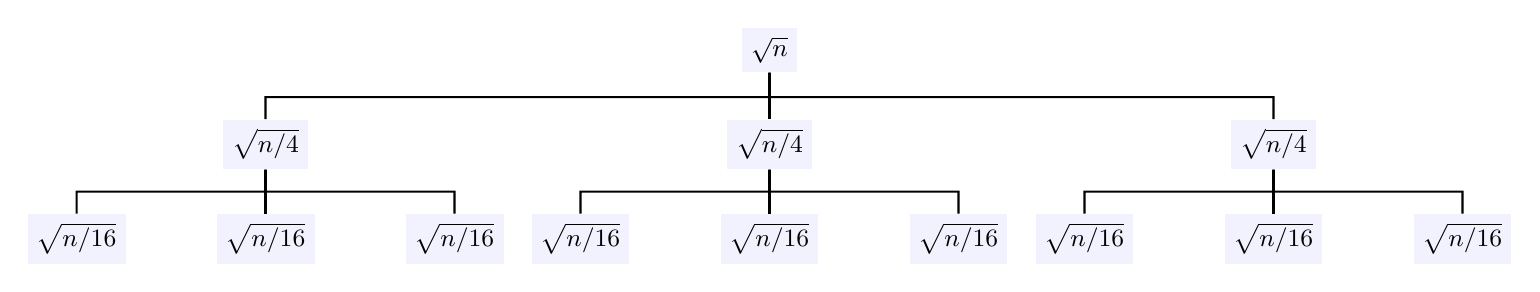
\begin{tikzpicture}[scale=0.8,font=\small, edge from parent fork down,
every node/.style={fill=blue!5},
edge from parent/.style={black,thick,draw},
level 1/.style={sibling distance=8cm},
level 2/.style={sibling distance=3cm}]
\node {$\sqrt{n}$}
      child {node {$\sqrt{n/4}$}
      child {node {$\sqrt{n/16}$}}
      child {node {$\sqrt{n/16}$}}
      child {node {$\sqrt{n/16}$}}
      }
 child {node {$\sqrt{n/4}$}
      child {node {$\sqrt{n/16}$}}
      child {node {$\sqrt{n/16}$}}
      child {node {$\sqrt{n/16}$}}
      }
 child {node {$\sqrt{n/4}$}
       child {node {$\sqrt{n/16}$}}
       child {node {$\sqrt{n/16}$}}
       child {node {$\sqrt{n/16}$}}
      };
\end{tikzpicture}
\newline
\newline
Erklärung zu a)
\newline
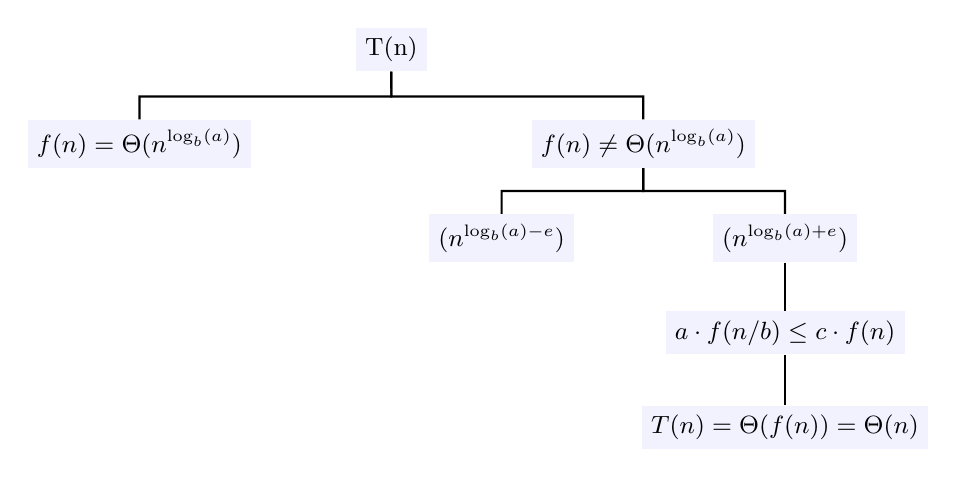
\begin{tikzpicture}[scale=0.8,font=\small, edge from parent fork down,
every node/.style={fill=blue!5},
edge from parent/.style={black,thick,draw},
level 1/.style={sibling distance=8cm},
level 2/.style={sibling distance=4.5cm}]
\node {T(n)} 
 child {node {$f(n) = \Theta(n^{\log_b(a)})$}}
 child {node  {$f(n) \neq \Theta(n^{\log_b(a)})$}
       child {node {$(n^{\log_b (a)-e})$}}
       child {node {$(n^{\log_b(a) + e})$}
             child {node {$a\cdot f(n/b) \leq c\cdot f(n)$} 
                   child {node {$T(n)=\Theta(f(n))=\Theta(n)$}}
             }
        }
    };
\end{tikzpicture}
\newline
Erklärung zu b)
\newline
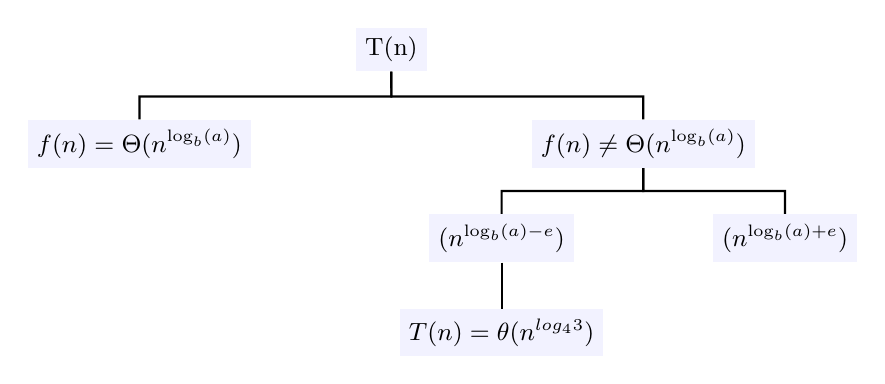
\begin{tikzpicture}[scale=0.8,font=\small, edge from parent fork down,
every node/.style={fill=blue!5},
edge from parent/.style={black,thick,draw},
level 1/.style={sibling distance=8cm},
level 2/.style={sibling distance=4.5cm}]
\node {T(n)} 
 child {node {$f(n) = \Theta(n^{\log_b(a)})$}}
 child {node  {$f(n) \neq \Theta(n^{\log_b(a)})$}
       child {node {$(n^{\log_b (a)-e})$}
             child {node {$T(n)= \theta (n^{log_43})$}}
       }
       child {node {$(n^{\log_b(a) + e})$}}
    };
\end{tikzpicture}
\end{flushleft}
\end{document}
